\documentclass[10pt]{beamer}

%\usetheme{ENSLyon}

\usetheme{AnnArbor}

\title[PIBIC 2021/2022]{\Large \textsc{Seminário I:\\ Álgebra Geométrica}}
\author[G. Philippi]{{Guilherme Philippi\vspace{-0.3cm}}}
\institute[]{Departamento de Matemática\\ Universidade Federal de Santa Catarina, Blumenau \\ \vspace{0.2cm} Orientado por Felipe Fidalgo\vspace{-0.2cm}}
\date[18 Fevereiro, 2022]{ {\small PIBIC ciclo 2021/2022 } \\ {\scriptsize Teoria e prática em Distance Geometry e Clifford Algebras com aplicações \\ 18 de fevereiro de 2022}}
\setbeamersize{text margin left=5mm}
\setbeamersize{text margin right=5mm}

\setbeamertemplate{navigation symbols}{}
%\usecolortheme{ENSLyon_greener}
\usecolortheme{whale}

\setbeamercolor{frametitle}{bg=gray}
\setbeamertemplate{bibliography item}{\insertbiblabel}

%PACKAGES -------------------------
\usepackage{etex}
\usepackage[utf8]{inputenc}
\usepackage[brazilian]{babel}
\usepackage{enumerate}
\usepackage{amsmath}
\usepackage{amssymb}
\usepackage{amsthm}
\usepackage{amscd}
\usepackage{amsfonts}
\usepackage{multicol}
\usepackage{multirow}
\usepackage{array}
\usepackage{color}
\usepackage{graphicx}
\usepackage{tikz}
\usepackage{tikz-qtree}
\usepackage{wrapfig}
\usepackage{3dplot}
\usepackage{pgf}
\usepackage{tkz-euclide}
\usepackage{algorithmic}
\usepackage{algorithm}
\usepackage{xparse}
\usepackage{subfigure}

%LIBRARIES-TIKZ ------------------------------------------

\usetikzlibrary{shadows,trees}
\usetikzlibrary{decorations.pathmorphing}
\usetikzlibrary{decorations.markings}
\usetikzlibrary{positioning}
\usetikzlibrary{chains,matrix,scopes}
\usetikzlibrary{arrows}

%DEFINITIONS ----------------------------------------------------

\def\centerarc[#1](#2)(#3:#4:#5)% Syntax: [draw options] (center) (initial angle:final angle:radius)
{ \draw[#1] ($(#2)+({#5*cos(#3)},{#5*sin(#3)})$) arc(#3:#4:#5); }
\def\xx{\mathbf{x}}
\def\ii{\mathbf{i}}
\def\jj{\mathbf{j}}
\def\kk{\mathbf{k}}
\def\tt{\mathbf{t}}
\def\ee{\mathbf{e}}
\def\qq{\mathbf{q}}
\def\pp{\mathbf{p}}
\def\vv{\mathbf{v}}
\def\rr{\mathbf{r}}
\def\vzero{\mathbf{0}}
\def\qset{\mathbb{H}}
\def\xx{\mathbf{x}}


\AtBeginSection[]
{
	\begin{frame}<beamer>
		\frametitle{Inicio da seção \thesection}
		\tableofcontents[currentsection]
	\end{frame}
}


%NEW THEOREMS ------------------------------------------

\theoremstyle{plain}
\newtheorem{teorema}{Teorema}[section]
\newtheorem{lema}{Lema}[section]
\newtheorem{proposicao}{Proposição}[section]
\newtheorem{corolario}{Corolário}[section]

\theoremstyle{definition}
\newtheorem{definicao}{Definição}[section]
\newtheorem{observacao}{Observação}[section]
\newtheorem{exemplo}{Exemplo}[section]

\newenvironment{solucao}
{\renewcommand\qedsymbol{$\triangle$}\begin{proof}[Solução]}{\end{proof}}



\begin{document}
	
	%FACE
	\begin{frame}
		
		\titlepage
		
		\vspace{-0.65cm}
		\begin{flushleft}
			
\includegraphics[scale=1.5]{logo.png}
		\end{flushleft}
		
		\vspace{-2cm}
		\begin{flushright}
			
\includegraphics[scale=0.024]{logo_ufsc.png}
		\end{flushright}
	\end{frame}
	
	%Indice
	\begin{frame}
		\tableofcontents 
	\end{frame}
	
	\section{Preliminares - recordar é viver}
	
	\begin{frame}
		\frametitle{Recordar é viver } 
		{
			\begin{definicao}[$R$-Módulo] Seja $(R,+,\cdot)$ um anel.
				Um grupo abeliano $(M,\oplus)$ é chamado de \emph{módulo sobre um anel $R$} (ou, simplesmente $R$-módulo) se existir uma aplicação
				$$
				\begin{tabular}{rcl}
					$R\times M$ & $\longrightarrow$ & $M$\\
					$(r,m)$ & $\mapsto$ & $rm$
				\end{tabular},
				$$
				chamada \emph{multiplicação por escalar}, tal que para todo $r,r'\in R$ e $m, m'\in M$ valham
				\begin{enumerate}
					\item $0_Rm = 0_M$;
					\item se $R$ tem identidade $1$, então $1m = m$;
					\item $(r+r')m = (rm)\oplus(r'm)$;
					\item $r(m\oplus m') = (rm)\oplus(rm')$;
					\item $(r\cdot r')m = r(r'm)$.
				\end{enumerate}
			\end{definicao}
		}	
	\end{frame}

	\begin{frame}
		\frametitle{Recordar é viver } 
		{
			
			\begin{exemplo}[$\mathbb{Z}$-módulo]
				Seja o anel $(\mathbb{Z}, +, \cdot)$. Podemos fazer qualquer grupo abeliano $(A,+)$ virar um $\mathbb{Z}$-módulo através do seguinte produto escalar: para $n\in \mathbb{Z}$ e $a\in A$,
				$$
				\begin{tabular}{rll}
					$na=$&
					$\left\{
					\begin{tabular}{l}
						$a + a + \cdots + a \quad (n\text{ vezes}),$\\
						$0$,\\
						$-a -a -\cdots -a \quad (-n\text{ vezes}),$
					\end{tabular}\right.$&
					\begin{tabular}{l}
						se $n>0$\\
						se $n=0$\\
						se $n<0$\\
					\end{tabular}
				\end{tabular}
				.$$
			\end{exemplo}
			
			\begin{definicao}[Espaço vetorial]
				Seja o grupo abeliano $E$ um $K$-módulo. Se $K$ é um corpo, dizemos que $E$ é um \emph{espaço vetorial sobre o corpo $K$}. Também, passamos a nos referenciar aos elementos de $K$ por \emph{escalares} e aos de $E$ por \emph{vetores}.
			\end{definicao}
			E assim ganhamos a possibilidade de ``contrair'' elementos de $E$, em relação a elementos de $K$ ``contraídos''.
		}	
	\end{frame}

	\section{Álgebra dos subespaços vetoriais com produto interno}
	\begin{frame}
		\frametitle{Espaços vetoriais com produto interno}
		
		
		
		
		
		Vamos incrementar os espaços vetoriais com uma aplicação adicional.
		
		\begin{definicao}[Espaço com produto interno]
			Seja $E$ um espaço vetorial sobre $K$. Um \textit{produto interno} sobre $E$ é uma função $\left <,\right>: E\times E \longrightarrow K$ tal que valham
			\begin{enumerate}
				\item \textit{(Positividade)} Para todo $v\in E$, $$\left <v,v\right > \geq 0 \quad \text{e} \quad \left <v,v\right > = 0 \iff v = 0;$$
				\item \textit{(Simetria)} Para todo $v,u \in E$, $\left <u,v\right > = \left <v,u\right >;\footnote{mais geralmente, quando $K$ é um corpo complexo, $\left <u,v\right > = \overline{\left <v,u\right >}$}$ 
				\item \textit{(Linearidade no primeiro argumento)} Para todo $v,u,w \in E$ e $r,s \in K$, $$\left < ru + sv, w\right > = r\left <u,w\right > + s\left <v,w \right >.$$
			\end{enumerate}
			O espaço vetorial $E$ sobre $K$, junto do produto interno $\left <,\right >$, é chamado \textit{$K$ espaço com produto interno}.
			
		\end{definicao}
	\end{frame}

	\begin{frame}
		\frametitle{Espaços vetoriais com produto interno: implicações}
		
		Se $K = \mathbb{R}$, então as propriedades (2) e (3) mostram que o produto interno é bilinear. Caso $K$ seja complexo, tem-se algo que chamamos linearidade conjugada, da forma $$\left < w,ru +sv\right > = \overline{\left < ru+sv, w \right >} = \overline{r}\left < w,u\right > + \overline{s}\left <w,v\right >.$$
		
		\begin{definicao}[Norma]
			A \textit{norma} de $v\in E$ é definida como $\lVert v\rVert = \sqrt{\left < v,v \right >}.$ 
		\end{definicao}
		
		\begin{proposicao}
			$\lVert v\rVert \geq 0$ e $\lVert v\rVert =0$ se, e somente se, $v = 0$.
		\end{proposicao}
		
		\begin{proposicao}
			Para todo $r \in K$ e $v \in E$, $$\lVert rv\rVert = \left|r\right| \lVert v\rVert.$$
		\end{proposicao}
	\end{frame}

	\begin{frame}
		\frametitle{Espaços vetoriais com produto interno: implicações}
		
		\begin{teorema}[Desigualdade de Cauchy-Schwarz]
			Para todo $u,v \in E$,
			$$\left|\left < u,v\right >\right| \leq \lVert u\rVert \lVert v\rVert$$
		\end{teorema}
	
		\begin{teorema}[Desigualdade triangular]
			$$\lVert u+v\rVert \leq \lVert u\rVert + \lVert v\rVert$$
		\end{teorema}
	
		\begin{proposicao}
			As igualdades dos teoremas acima só acontecem quando $v = \alpha u$, com $\alpha\in K$.
		\end{proposicao}
	
		\begin{teorema}[A lei do paralelogramo]
			Para todo $u,v\in E$, $$\lVert u+v\rVert^2 + \lVert u-v\rVert^2 = 2\lVert u\rVert^2 + 2\lVert v\rVert^2$$
		\end{teorema}
	\end{frame}

	\section{Espaços métricos}
	
	\begin{frame}
		\frametitle{Espaços métricos}
		
		\begin{definicao}[Espaço métrico]
			Chamamos de \textit{espaço métrico} um espaço com produto interno $M$ sobre $\mathbb{R}$, monido de uma função $d: M\times M \longrightarrow \mathbb{R}$, que associa pares de vetores a um número real que chamamos de distância entre esses pontos, tal que valham, $\forall \ u,v,w \in M$,
			\begin{enumerate}
				\item $d(u,v) \geq 0$ e $d(u,v) = 0 \iff u = v$; 
				\item $d(u,v) = d(v,u)$;
				\item $d(u,v) \leq d(u,w) + d(w,v)$.
			\end{enumerate}
		\end{definicao}
	
		\begin{exemplo}
			Seja $d(u,v)$ a distância entre os dois vetores $u$ e $v\in E$ definida como $$d(u,v) = \lVert u-v\rVert.$$
		\end{exemplo}
	\end{frame}

	\begin{frame}
		\frametitle{Pseudométricas}
		
		\begin{definicao}[Espaço pseudométrico]
			Chamamos de \textit{espaço pseudométrico} um espaço com produto interno $M$ sobre $\mathbb{R}$, monido de uma função de distância $d: M\times M \longrightarrow \mathbb{R}$, tal que valham, $\forall \ u,v,w \in M$,
			\begin{enumerate}
				\item $d(u,v) \geq 0$ e $u = v \implies d(u,v) = 0 $; 
				\item $d(u,v) = d(v,u)$;
				\item $d(u,v) \leq d(u,w) + d(w,v)$.
			\end{enumerate}
		\end{definicao}
	
		\begin{proposicao}
			Um espaço pseudométrico é métrico se, e somente se, $d(u,v) > 0$ sempre que $u\neq v$.
		\end{proposicao}
		
	\end{frame}
	
	\begin{frame}
		\frametitle{Assinatura de uma métrica}
		
		Uma maneira prática para representar uma métrica $Q$ é pelo uso de uma \textbf{matriz de métrica} $M$, ou tensor métrico, 
		
		\begin{center}
			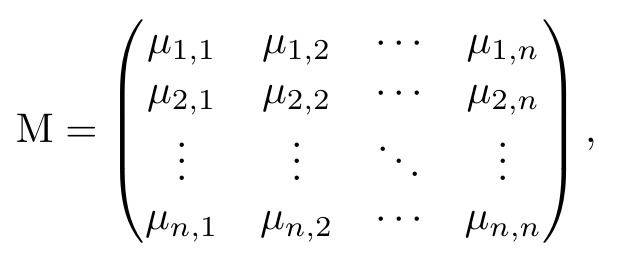
\includegraphics[width=0.35\linewidth]{figures/metricaQ.png}	
		\end{center}
		\vspace{-0.3cm}
		simétrica que codifica a distância entre os pares dos vetores de base $\{e_i\}_{i=1}^n$ do espaço métrico, \textit{i.e.}, $\mu_{i,j} = d(e_i,e_j)$, para $1\leq i, \ j\leq n$.
		
		Perceba que quando $d(e_i,e_j) = \lVert e_i-e_v
	\end{frame}
	
	
	\section{Álgebra Geométrica}
	\begin{frame}
		\frametitle{Álgebra Geométrica: introdução}
		\begin{center}
			espaço físico $\times$ espaço de representação
		\end{center}
		O espaço de representação da \textbf{Álgebra Linear} é construída a partir do \textbf{conceito de vetor}, isso é, \textbf{pontos no espaço de representação}. 
		
		Já a \textbf{Álgebra Geométrica} é construída sobre o conceito de \textbf{subespaços vetoriais}, o que implica uma nova natureza de seus objetos elementares.
		\vspace{0.5cm}
		
		A partir das ideias de \textbf{Grassmann}, com sua Álgebra Exterior, \textbf{pode-se codificar elementos de dimensões variadas}, produto dos elementos de sua própria álgebra. Combinando este produto de Grassmann com o produto interno (clássico da álgebra linear), \textbf{dá-se origem a um novo produto}, capaz de codificar transformações nesse novo espaço de maneira \textbf{muito mais simples} (eficiente?) do que na Álgebra Linear. 
		
		Não só, mas esse novo produto \textbf{permite interpretar tais transformações (operadores) como objetos geométricos e vice versa}!
	\end{frame}

	\begin{frame}
		\frametitle{Álgebra Geométrica: introdução}
		\vspace{-1cm}
		\begin{figure}[H]
			\hspace{-6cm}
			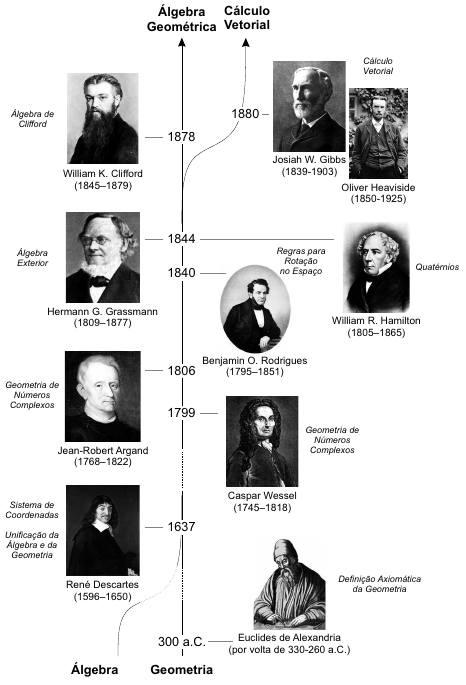
\includegraphics[width=0.4\linewidth]{figures/GAcronologia.png}
			\label{fig:cronologia}
		\end{figure}
		\tiny Cronologia das descobertas, incluindo os cientistas que mais influenciaram \\no desenvolvimento da Álgebra Geométrica.
	
		\vspace{-6cm}
		
		\begin{figure}[H]
			\hspace{6cm}
			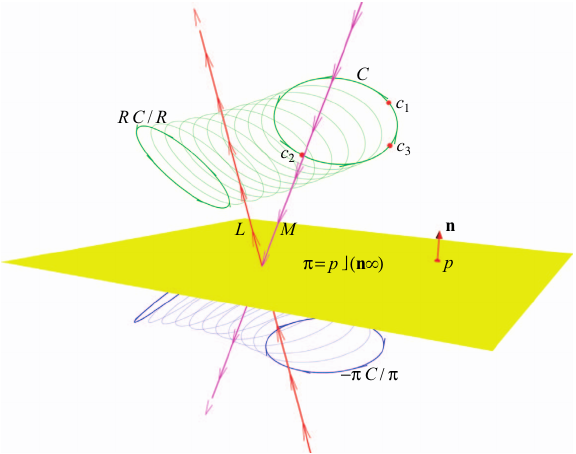
\includegraphics[width=0.4\linewidth]{figures/whyGA.png}
			\label{fig:lable}
		\end{figure}
	
		\hspace{6cm}
		A rotação do círculo $C$ (determinado por três pontos $c_1,c_2$ e $c_3$) \\
		\hspace{6cm} ao redor da linha $L$, e suas reflexões através de um plano $\Pi$.
	\end{frame}

	\begin{frame}
		\frametitle{Subespaços orientados como primitivas: o produto externo}
		
		Em Álgebra Linear, assumindo base $\{e_i\}^n_{i=1}$ para $\mathbb{R}^n$, um vetor $a$ arbitrário pode ser escrito como a \textit{combinação linear} dos elementos da base. Para $n=3$, $$a = \alpha_1e_1 + \alpha_2e_2 + \alpha_3e_3\in \mathbb{R}^3$$
		
		\begin{figure}[H]
			\hspace{-5cm}
			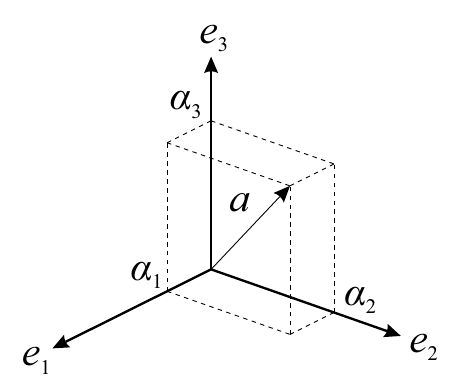
\includegraphics[width=0.4\linewidth]{figures/aR3.png}
		\end{figure}
		
		\vspace{-3.7cm}
		\begin{figure}[H]
			\hspace{5cm}
			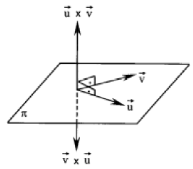
\includegraphics[width=0.3\linewidth]{figures/produtoVetorial.png}
		\end{figure}
		
		
		Na Álgebra Linear temos o produto vetorial, limitado a vetores no $\mathbb{R}^3$, onde um o produto de dois vetores $\vec u,\vec v\in \mathbb{R}^3$ gera um novo vetor $\vec u \times \vec v\in \mathbb{R}^3$ perpendicular aos outros dois.\\
		Uma dúvida natural é: existe algum produto que generalize o produto vetorial para qualquer dimensão?
		
	\end{frame}

	\subsection{Subespaços orientados como primitivas: o produto externo}
	\begin{frame}
		\frametitle{Subespaços orientados como primitivas: o produto externo}
		
		Grassmann define um produto que nos permite construir subespaços de dimensionalidade mais alta a partir de vetores:
		o \textbf{produto externo} $b\wedge a$ entre os vetores $b$ e $a$ pode ser usado para representar o subespaço 2-dimensional
		\begin{figure}[H]
			\vspace{0.5cm}
			\hspace{-5cm}
			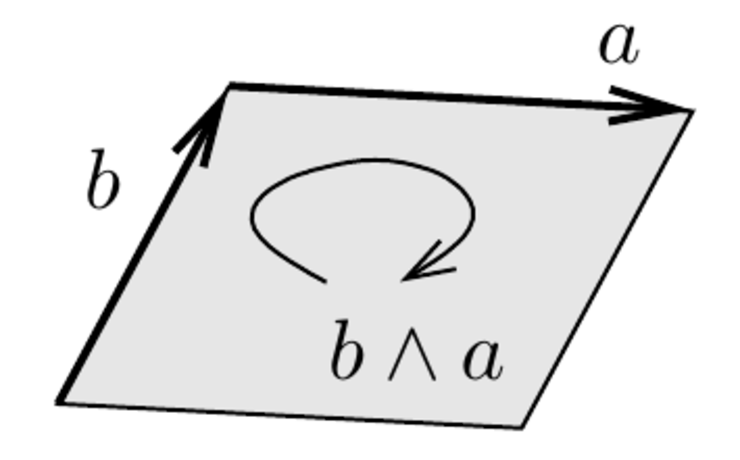
\includegraphics[width=0.3\linewidth]{figures/2blade2.pdf}
		\end{figure}
	
		\vspace{-3cm}
		\begin{figure}[H]
			\hspace{5cm}
			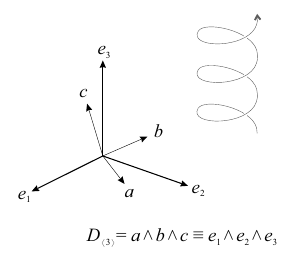
\includegraphics[width=0.3\linewidth]{figures/d3.png}
		\end{figure}
	
		No geral, em Álgebra Geométrica, podemos gerar tais subespaços com dimensão $k$ a partir de $k$ vetores linearmente independentes em $\mathbb{R}^n$. Chamamos tais subespaços de \textbf{$k$-blades}, onde $k$ é o \textbf{grau} do blade. Estes serão os elementos primitivos da Álgebra Geométrica. Veja que isso generaliza a Álgebra Vetorial, onde possuíamos apenas os 0-blades e 1-blades, isso é, escalares e vetores. 
	\end{frame}

	\begin{frame}
		\frametitle{O espaço Multivetorial $\bigwedge \mathbb{R}^n$}
		Assim, a partir dos elementos do espaço vetorial $\mathbb{R}^n$, \textbf{podemos construir um espaço multivetorial} $\bigwedge\mathbb{R}^n$. Isso é, temos $\sum_{k=0}^{n} {n\choose k} = 2^n$ $k$-combinações dos vetores de base de $\mathbb{R}^n$, que descrevem $2^n$ \textbf{blades de base} para $\bigwedge\mathbb{R}^n$. No caso $n =3$, temos
		
		\begin{figure}[H]
			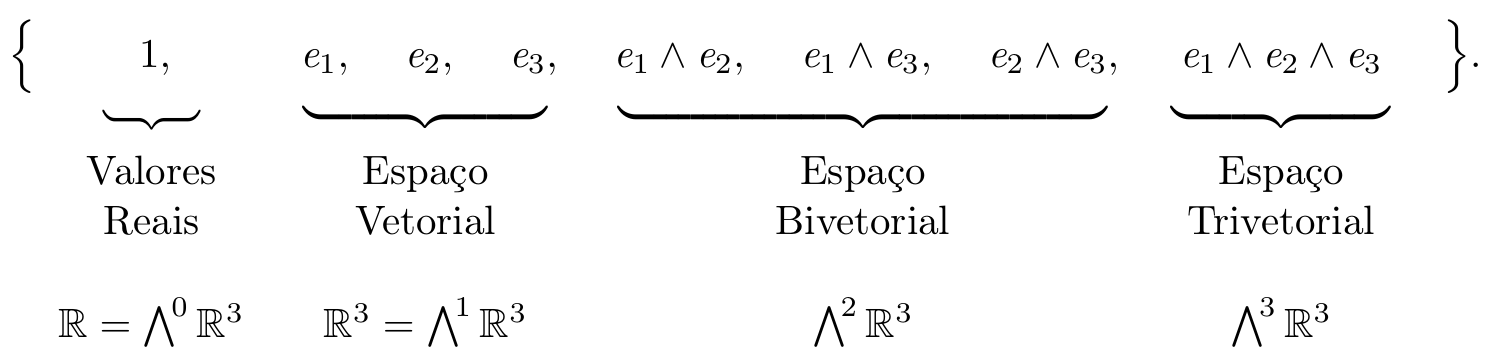
\includegraphics[width=0.8\linewidth]{figures/wr3.png}
		\end{figure}
		
		A combinação linear destes elementos formam os \textbf{multivetores}.
		\vspace{0.2cm}
		
		\begin{minipage}{0.68\linewidth}
			Perceba a simetria entre $\bigwedge^k\mathbb{R}^n$ e $\bigwedge^{n-k}\mathbb{R}^n$.
			
			Por conta de tal simetria, chamamos os elementos de $\bigwedge^{n-1}\mathbb{R}^n$ de \textbf{pseudovetores} e os elementos de $\bigwedge^{n}\mathbb{R}^n$ de \textbf{pseudoescalares}.	
		\end{minipage}
		\vspace{-2.4cm}
		\begin{figure}[H]
			\hspace{9cm}
			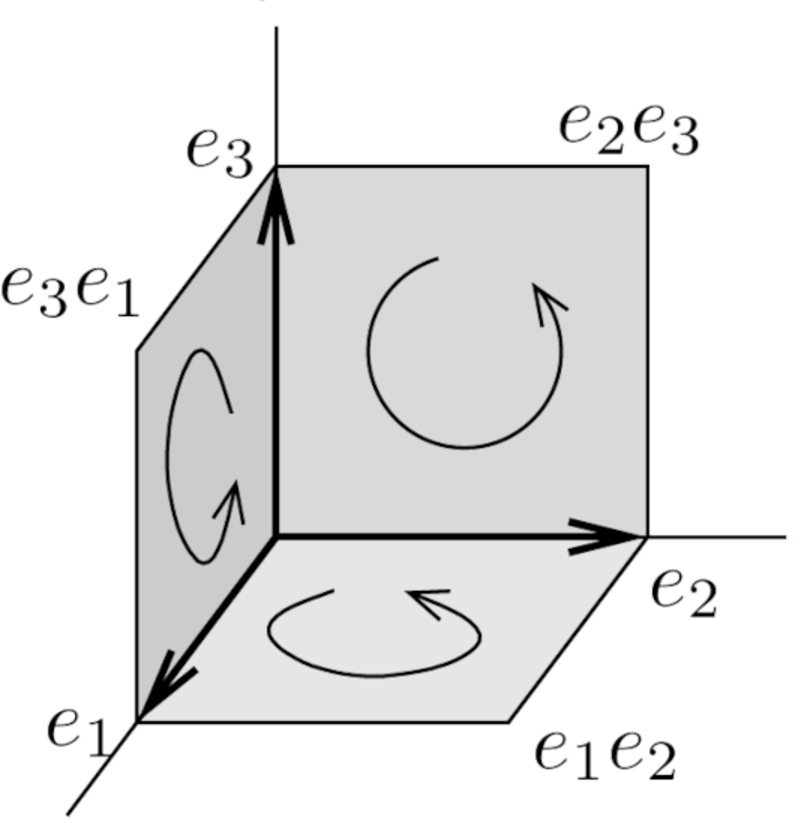
\includegraphics[width=0.2\linewidth]{figures/bivectorsBase.pdf}
		\end{figure}
		\vspace{-0.2cm}
		Assim, um 2-\textbf{vetor} (não necessáriamente 2-blade) pode ser escrito como \vspace{-0.18cm}$$C_{\left < 2\right >} = \alpha_1 e_1\wedge e_2 + \alpha_2 e_1 \wedge e_3 + \alpha_3 e_2 \wedge e_3$$. 
	\end{frame}

	\begin{frame}
		Conhecendo o espaço multivetorial $\bigwedge\mathbb{R}^n$ podemos definir formalmente o produto externo, como o mapeamento:
		\begin{figure}[H]
			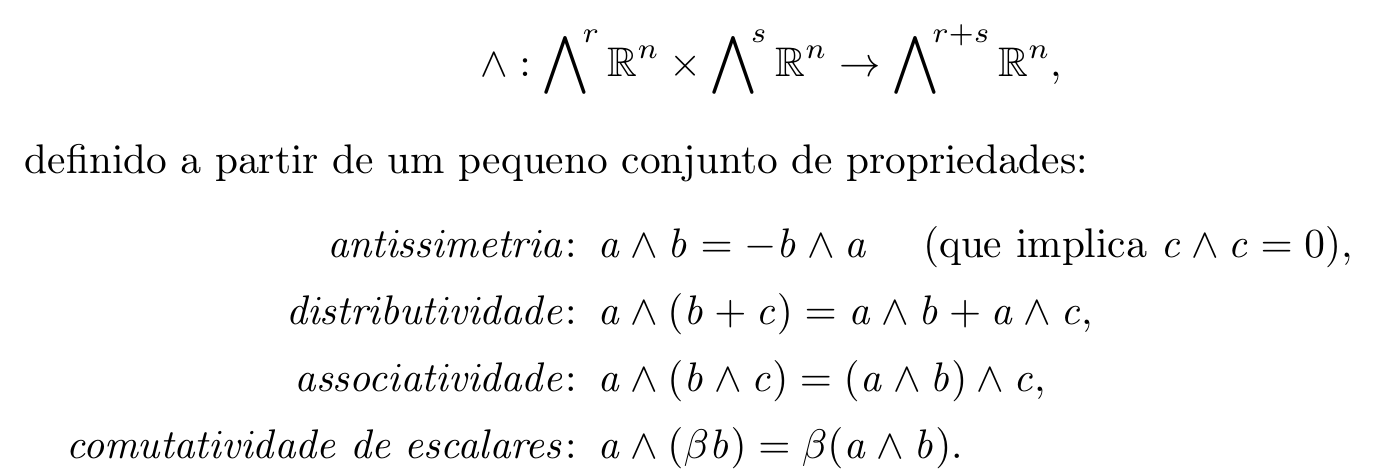
\includegraphics[width=0.9\linewidth]{figures/externalProduct.png}
		\end{figure}
	\end{frame}

	\subsection{O produto regressivo}
	
	\begin{frame}
		\frametitle{O produto regressivo}
		Com o \textbf{produto regressivo} podemos construir subespaços orientados $k$-dimensionais a partir de $(n-k)$ pseudovetores. Por exemplo, para $n=3$, $c = A_{\left <2\right >} \vee B_{\left <2\right >}$
		
		\vspace{0.5cm}
		\begin{minipage}{0.8\linewidth}
			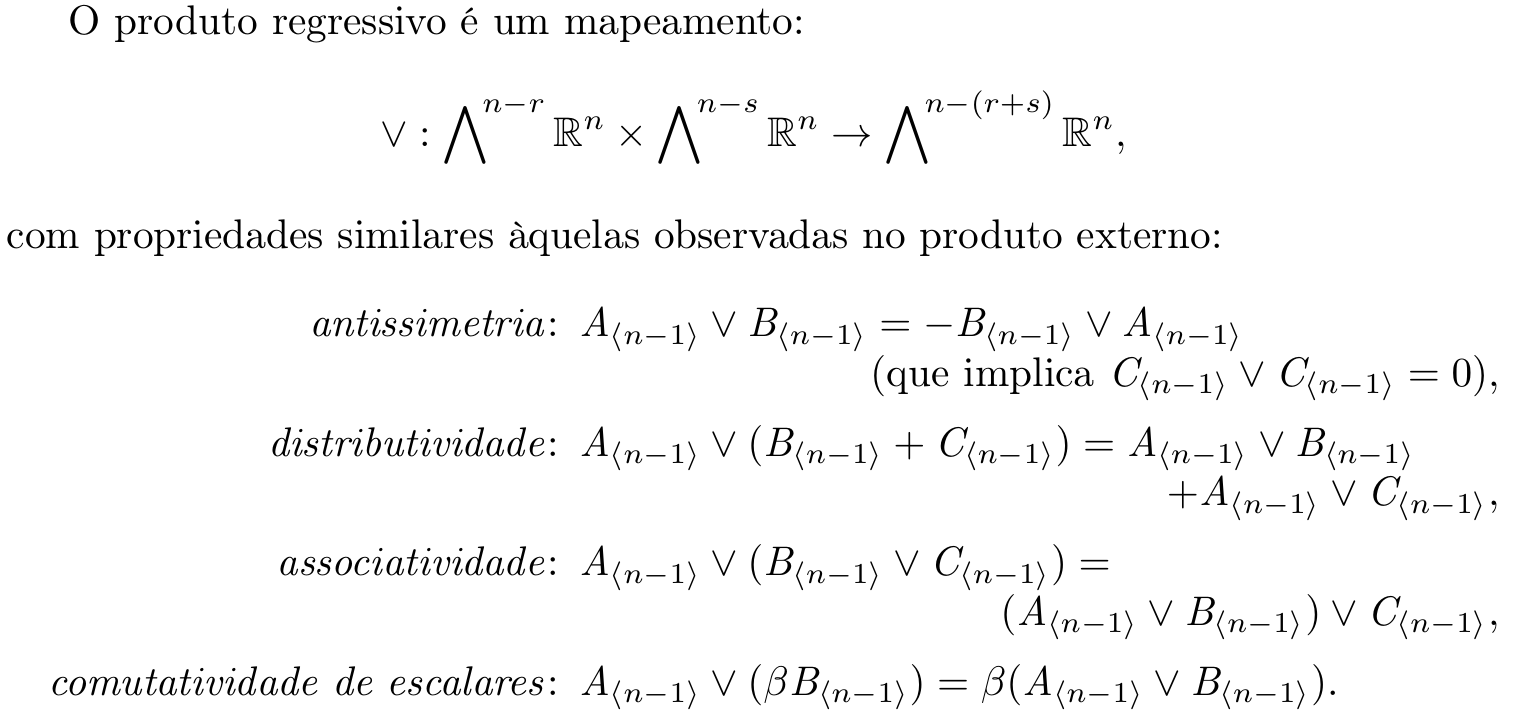
\includegraphics[width=1\linewidth]{figures/produtoRegressivoDef.png}
		\end{minipage}
		\begin{minipage}{0.18\linewidth}
			\vspace{-3cm}
			\hspace{-1cm}
			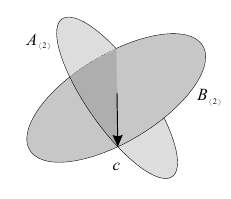
\includegraphics[width=1.2\linewidth]{figures/produtoRegressivo.png}
		\end{minipage}
	
		\vspace{0.3cm}
		Perceba que o produto regressivo é calculado encontrando o subespaço $C_{\left <t\right >}$ compartilhado por $A_{\left <r\right >}$ e $B_{\left <s\right >}$. Isso pode ser algo complicado fora da AG.
	\end{frame}
	
	
	\subsection{O produto escalar de Blades}
	
	
	\subsection{Contrações}
	
	\subsection{O produto Geométrico}
	%\section{Álgebra Exterior e blades em um espaço vetorial}
	
	\subsection{Dualidade}
	
	\section{Modelos de Geometria}
	
	\subsection{Modelo Euclidiano}
	
	\subsection{Modelo Homogêneo}
	
	\subsection{Modelo Conforme}
	
	
	\section{Referências}
	%Slide refe
	\begin{frame}		
		
		{\footnotesize
		\bibliographystyle{unsrt}
		\bibliography{references}}
	\end{frame}
	
	%Slide End
	\begin{frame}
		\begin{center}
			\vspace{1.5cm}
			Obrigado!\\
			\hspace{-5.5cm}
			
\includegraphics[scale=2.2]{logo.png}
			
			\vspace{-2.7cm}
			\hspace{5.5cm}
			
\includegraphics[scale=0.038]{logo_ufsc.png}
			
			\vspace{0.5cm}
			Contato: g.philippi\@grad.ufsc.br\\ UFSC - Blumenau
		\end{center}
	\end{frame}
	
\end{document}